%\documentclass[12pt]{scrbook}
%
%\usepackage{tikz}
%\usepackage{minted}
%\usetikzlibrary{decorations.pathreplacing,arrows}
%
%\usepackage{fullpage}
%\usepackage{subfigure}
%\begin{document}
%
%
%Lorem Ipsum is simply dummy text of the printing and typesetting industry. Lorem Ipsum has been the industry's standard dummy text ever since the 1500s, when an unknown printer took a galley of type and scrambled it to make a type specimen book. It has survived not only five centuries, but also the leap into electronic typesetting, remaining essentially unchanged. It was popularised in the 1960s with the release of Letraset sheets containing Lorem Ipsum passages, and more recently with desktop publishing software like Aldus PageMaker including versions of Lorem Ipsum.

\begin{figure}
\centering

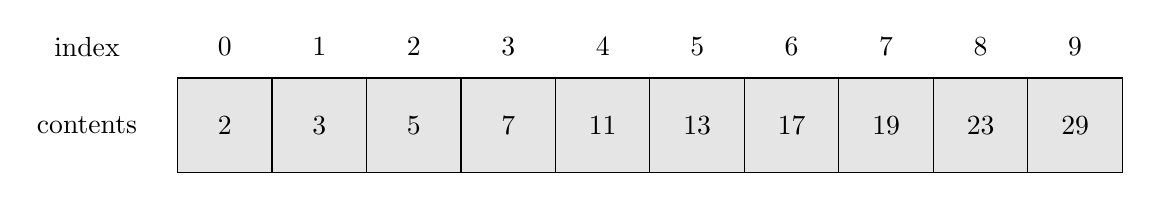
\begin{tikzpicture}
% size of each node
\def\sz{12mm}
% node style definition
\tikzstyle{block} = [
	draw, fill=black!10, rectangle,
	minimum height=\sz, minimum width=\sz ];
\tikzstyle{plain} = [draw=none,fill=none];
% array element definition
\def\arr{2, 3, 5, 7, 11, 13, 17, 19, 23, 29 };
%\def\x{0}; % x pos of arr
%\def\y{0}; % y pos of arr
\newcounter{ind};
\setcounter{ind}{0};
\node[plain] at (-1.75, 1) { index };
\node[plain] at (-1.75, 0) { contents };
\foreach \item in \arr
{
	\node[block] at (\theind*\sz,0) { \item };
	\node[plain] at (\theind*\sz,1.0) { \theind };
	\addtocounter{ind}{1};
}
\end{tikzpicture}

\caption[Example of an Array]{An integer array of size 10.  Using zero-indexing, the first
element is at index 0, the last at index 9.}
\label{figure:arrayExample}
\end{figure}

%\end{document}

